\chapter{Mimicking Portfolio}

This approach uses purely statistical methods to choose the 
portfolio weights, and does not rely on any economic priors.

\section{Random Variables}

We model stock returns as \textit{random variables}.
A random variable can take one of many values, with an 
associated probability. For example, the gross return on 
a stock can be one of four values as shown in Table \ref{tab:randomvariable}.

\begin{table}[!htbp]
    \centering
    \begin{tabular}{c c}
        % \hline
        $R$ & $P(R)$ \\
        % \hline
        1.1 & 0.6 \\
        1.2 & 0.1 \\
        0.7 & 0.25 \\
        0.0 & 0.05 \\
    \end{tabular}
    \caption{Example of a gross return distribution.}
    \label{tab:randomvariable}
\end{table}

Each value is a possible \textit{realization}
of the random variable. You can experiment with this in Python
using the following code:

\begin{python}
import numpy as np

# Define the possible returns and their probabilities
returns = np.array([1.1, 1.2, 0.7, 0.0])
probabilities = np.array([0.6, 0.1, 0.25, 0.05])

# Generate a random return
print(np.random.choice(returns, size=1, p=probabilities))

\end{python}

Of course, stock returns can take on many more values 
than just four, but this is a simple example.

The \textit{distribution} of the random variable is 
a listing of the values it can take, along with their
associated probabilities. For example, the distribution
of the random variable in Table \ref{tab:randomvariable}
is:

\begin{figure}[!htbp]
    \centering
    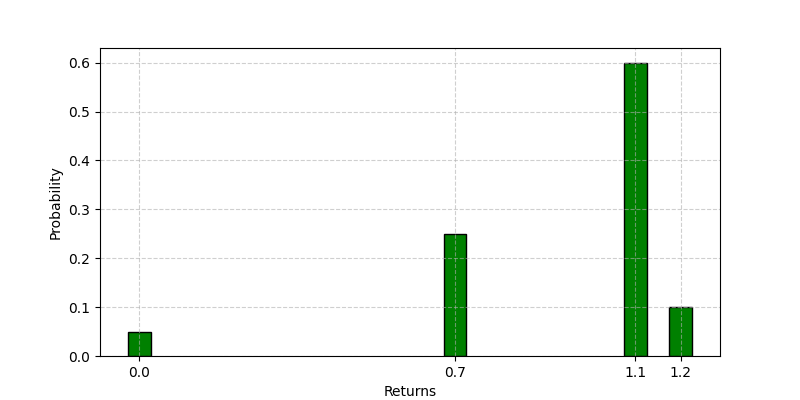
\includegraphics[width=0.8\textwidth]{mimicking/fig1.png}
    \caption{Example of a random variable distribution.}
    \label{fig:randomvariable}
\end{figure}





\section{Regression}

We will run regression, for example of a return 
on the market return:

\begin{equation}
    \label{eq:regression}
    R_t = \alpha + \beta R_{m,t} + \epsilon_t
\end{equation}

where $R_t$ is the return on the asset, $R_{m,t}$ is the return on the market
portfolio, $\alpha$ is the intercept, $\beta$ is the slope coefficient and
$\epsilon_t$ is the regression residual.

We may sometimes run multiple regressions of returns on the return
of several portfolios, for example:

\begin{equation}
    \label{eq:multiregression}
    R_t = \alpha + \beta R_{m,t} + \gamma R_{p,t} + \epsilon_t
\end{equation}

where $R_p$ is the return on the portfolio of interest.

The generic form is:

\begin{equation}
    \label{eq:genericregression}
    y_t = \alpha + \beta_1 x_{1,t} + \beta_2 x_{2,t} + \ldots + \beta_n x_{n,t} + \epsilon_t
\end{equation}

\subsection{$\beta$ estimation}

Starting with:

\begin{equation}
y_t = \alpha + \beta x_t + \epsilon_t
\end{equation}

With the usual assumption that errors are uncorrelated, we have 
the right hand variables $E(\epsilon_t x_t) = 0$ and $E(\epsilon_t) = 0$.

Multiplying both sides by $x_t - E(x_t)$ and taking expectations:


\begin{equation}
    \label{eq:population}
    \beta = \frac{Cov(y,x)}{Var(x)}
\end{equation}


\section{Mimicking the Market Portfolio}


\section{Time Series}

\section{Tracking Portfolio for News}

\section{Climate Hedge Target}

\section{Climate Risk Mimicking Portfolio}

The mimicking portfolio approach combines a pre-determined set of 
assets into a portfolio that is maximally correlated with a given 
climate change shock, using historical data. To obtain the mimicking
portfolios, we estimate the following regression model:

\begin{equation}
    \label{eq:regression}
    CC_t = w R_t + \epsilon_t
\end{equation}

where $CC_t$ denotes the (mean zero) climate hedge target in month $t$,
$w$ is a vector of $N$ portfolio weights, $R_t$ is the $N \times 1$ vector 
of demeaned excess returns and $\epsilon_t$ is the regression residual.
The portfolio weights are estimated each month using a rolling window of
$T$ months of historical data. 

% \begin{python}
%     if transactions: Transaction.create_transactions() # if transactions = "true"
%     node.generate_emptyState() # empty state for all nodes
%     S.initial_events() # initiate initial events to start with
    
%     while not queue.isEmpty() and clock <= targetTime:
%           next_e = queue.get_next_event()
%           clock = next_e.time # move clock to the time of the event
%           Event.execute_event(next_e)
%           Queue.remove_event(next_e)
    
%     print results
% \end{python}

\section{Conclusion}